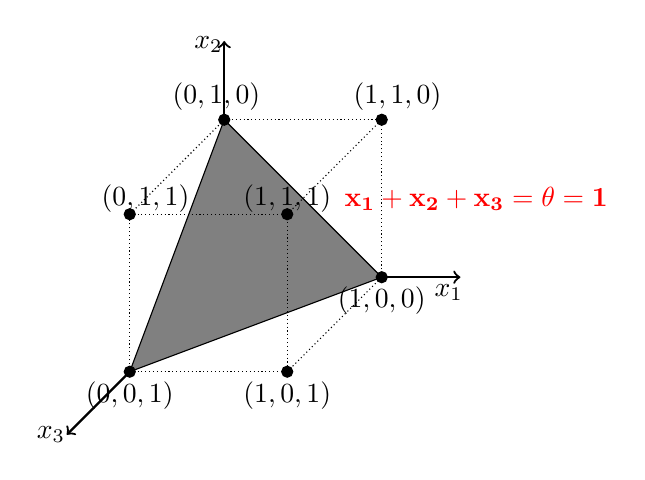
\begin{tikzpicture}

	\draw[thick,->] (0,0) -- (3.0,0);
	\draw[thick,->] (0,0) -- (0,3.0);
	\draw[thick,->] (0,0) -- (-2.0,-2.0);


	\node at (2.85, -0.2) {$x_1$};
	\node at (-0.2, 2.95) {$x_2$};
	\node at (-2.2, -2.0) {$x_3$};

	\node at (-0.1, -0.3) {$(0,0,0)$};
	\filldraw[fill=red] (0,0) circle (2pt);

	\only<5->{\draw[black, fill=gray] (2,0) -- (0,2) -- (-1.2,-1.2) -- (2,0) -- cycle;}

	\node at (-0.1, 2.3) {$(0,1,0)$};
	\node at (2.0, -0.3) {$(1,0,0)$};
	\node at (2.2, 2.3) {$(1,1,0)$};
	\node at (-1.2,-1.5) {$(0,0,1)$};
	\node at (0.8,-1.5) {$(1,0,1)$};
	\node at (-1.0,1.0) {$(0,1,1)$};
	\node at (0.8,1.0) {$(1,1,1)$};
	\onslide<5->{\node at (3.2, 1.0) {\color{red}{$\mathbf{x_1 + x_2 + x_3 = \mathbf{\theta} = 1}$}};}

	\filldraw (0,2) circle (2pt);
	\filldraw (2,0) circle (2pt);
	\filldraw (2,2) circle (2pt);
	\filldraw (-1.2,-1.2) circle (2pt);
	\filldraw (-1.2,0.8) circle (2pt);
	\filldraw (0.8,-1.2) circle (2pt);


	\draw[densely dotted] (0, 2) -- (-1.2,0.8);
	\draw[densely dotted] (-1.2,-1.2) -- (-1.2,0.8);
	\draw[densely dotted] (0.0,2.0) -- (2,2);
	\draw[densely dotted] (2.0,0.0) -- (2,2);
	\draw[densely dotted] (0.8,0.8) -- (2,2);
	\draw[densely dotted] (0.8,0.8) -- (0.8,-1.2);
	\draw[densely dotted] (0.8,-1.2) -- (2,0);
	\draw[densely dotted] (-1.2,-1.2) -- (0.8,-1.2);
	\draw[densely dotted] (-1.2,0.8) -- (0.8,0.8);


	\filldraw (0.8,0.8) circle (2pt);

\end{tikzpicture}